The term \textbf{\gls{kem}} indicates a category of key transport protocols (\Cref{sec:key_management:lifecycle:pre}). Differently from direct asymmetric encryption (\Cref{figure:kem}), a \gls{kem} expects a party to generate a random sequence of bytes whose length corresponds exactly to the length of a block of a given asymmetric cipher (such as \gls{rsa} --- see \Cref{sec:asymmetric_cryptography:ciphers}) --- hence, avoiding the risks of using padding (\Cref{algorithm:kem}). The random sequence of bytes will be fed to a \gls{kdf} (\Cref{sec:key_management:lifecycle:pre}) --- possibly along with further contextual data --- to derive a symmetric key which will be used for the actual data encryption (\Cref{sec:symmetric_cryptography}). The random sequence of bytes --- from now on called \textbf{encapsulated key} --- is encrypted with the recipient's public key. In this way, the recipient can decrypt the random sequence of bytes using the corresponding private key and derive the same symmetric key.

\remarkBlock{\gls{kem} freshness}{A generic \gls{kem} generates --- or, better, is supposed to generate --- a fresh symmetric key every time, since it involved the generation of a random sequence of bytes at every run.}

\lstinputlisting[
caption=Key Encapsulation Mechanism, 
label={algorithm:kem}, 
language=Python,
]{
	resources/code/kem.pseudocode
}

\begin{figure}[t!]
	\begin{center}
		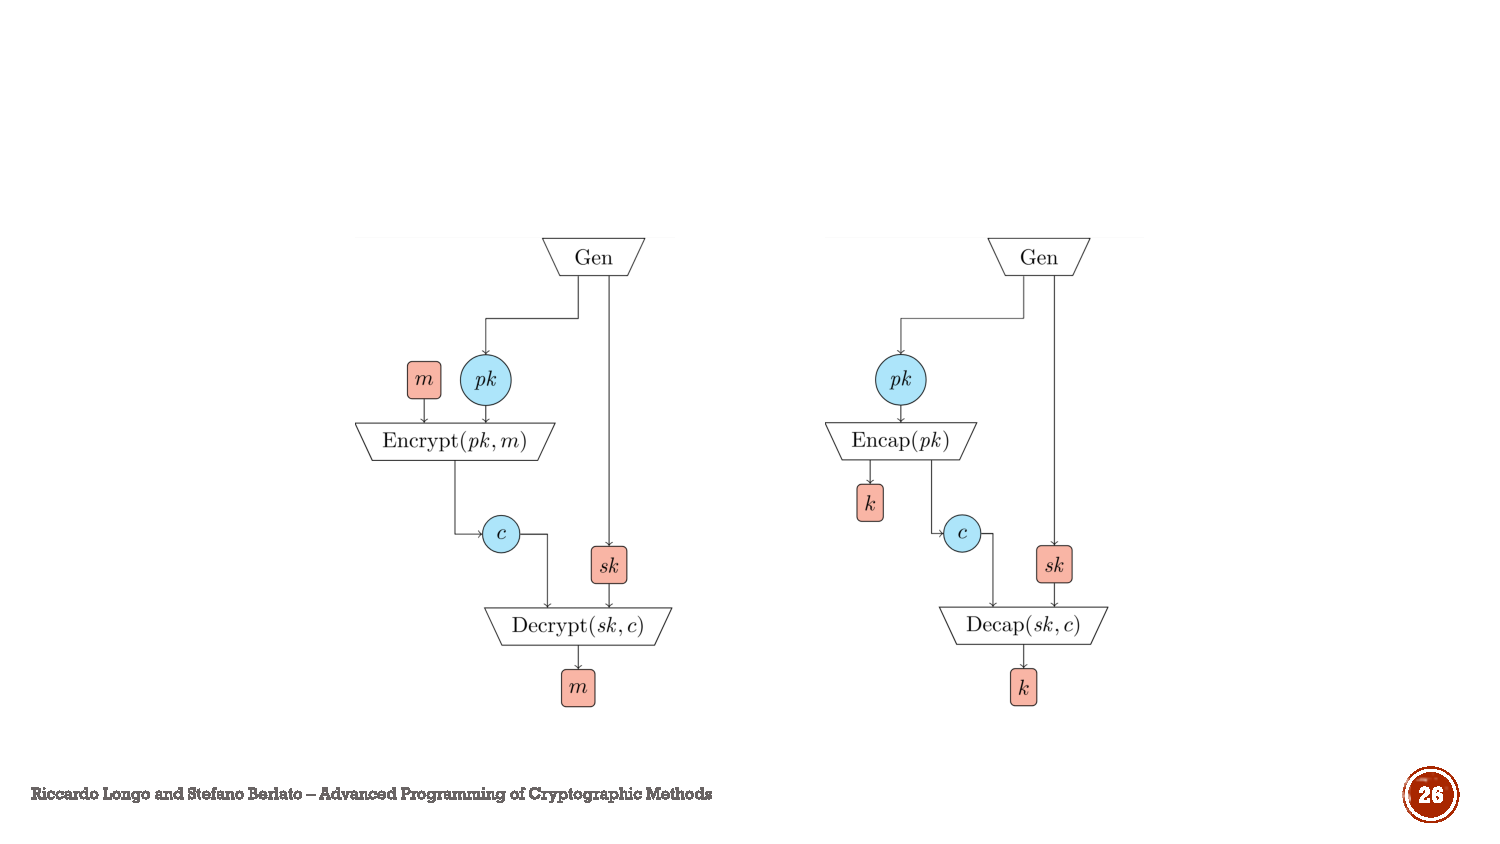
\includegraphics[trim={5.5cm 2cm 5.5cm 3cm},clip,width=0.75\linewidth]{resources/pdf/kem.pdf}
		\caption{Direct asymmetric encryption (on the left) vs. \gls{kem} (on the right) --- from \url{https://en.wikipedia.org/wiki/Key_encapsulation_mechanism}}
		\label{figure:kem}
	\end{center}
\end{figure}

\remarkBlock{\gls{dh} vs. \gls{kem}}{\gls{dh} (\Cref{sec:diffie_hellman}) is an instance of key agreement protocol, while a \gls{kem} pertains to key transport protocols (hence, as shown in \Cref{figure:key_generation_relationship}, both \gls{dh} and \glspl{kem} relate to key establishment). The main difference between \gls{dh} and \glspl{kem} is that \gls{dh} \textbf{typically} expects both parties to contribute to the symmetric key derivation with random or private values --- and only by combining both contributions can the shared secret be computed. Differently, \glspl{kem} expect one party only (the sender) to contribute with random or private values (as the recipient's public key is long-term, thus static) to derive a fresh symmetric key, encrypt (a precursor of) the symmetric key with the recipient's public key, and send the resulting ciphertext to the other party (the recipient); only at this point can the recipient decrypt (the precursor of) the symmetric key. Although it is true that \textbf{semi-ephemeral \gls{dh} (i.e., ephemeral-static mode) is practically equivalent to a \gls{kem}}, the concepts of \gls{dh} and \glspl{kem} are in general distinguished.}

\warningBlock{\gls{kem} and the \gls{kci} attack}{Straightforward \glspl{kem} --- in which only the public key of the recipient is used --- are vulnerable to the \gls{kci} attack (\Cref{sec:security_of_cryptographic_protocols}).}


\subsection{Authenticity in Key Encapsulation Mechanisms}\label{sec:key_encapsulation_mechanisms:authenticity}

Straightforward \glspl{kem} provide confidentiality but not sender authenticity. In other words, anyone can produce a valid ciphertext knowing the recipient's public key. To provide sender authenticity, the sender may either ($i$) create a digital signature of the ephemeral public key, the encapsulated key, or the symmetric key with a long-term key associated with the sender's identity (although this forces non-repudiation) --- see \Cref{sec:binding_keys_to_parties} --- or ($ii$) include the output of static-static or static-ephemeral \gls{dh} mode in the derivation of the symmetric key \footnote{\url{https://soatok.blog/2020/04/21/authenticated-key-exchanges/}} --- hence, use \gls{dh} instead of a \gls{kem}.


\subsection{Key Encapsulation Mechanisms with Multiple Recipients}\label{sec:key_encapsulation_mechanisms:multiple}

A \gls{kem} may be used to transport the same symmetric key to multiple recipients by leveraging key wrapping (\Cref{sec:cryptography_basics:keys}). In other words, the sender generates a random symmetric key, and then wraps it separately for each recipient. Hence, (the symmetric keys derived from) the encapsulated keys are used as \glspl{kek} rather than for directly encrypting data.

\readBlock{More information on key encapsulation mechanisms}{Soatok's blog post ``KEM Trails --- Understanding Key Encapsulation Mechanisms'' --- available at the link \url{https://soatok.blog/2024/02/26/kem-trails-understanding-key-encapsulation-mechanisms/} --- is an excellent supplementary resource for \glspl{kem}.}
